\chapter{Systematisches Konzept}

Das Blockschaltbild in Abbildung \ref{fig:blockschaltbild} zeigt den prinzipiellen Aufbau. Die Signale des SDR werden mit einem 1.5 GHz signal gemischt um sie entweder hoch oder runter zu transferrieren.

Dabei gilt der Zusammenhang

\begin{align}
    f_{\text{LO}} = k f_{\text{RF}} \pm f_{\text{IF}}, \quad k \in \mathbb{Z}
\end{align}

\begin{figure}
    \centering
    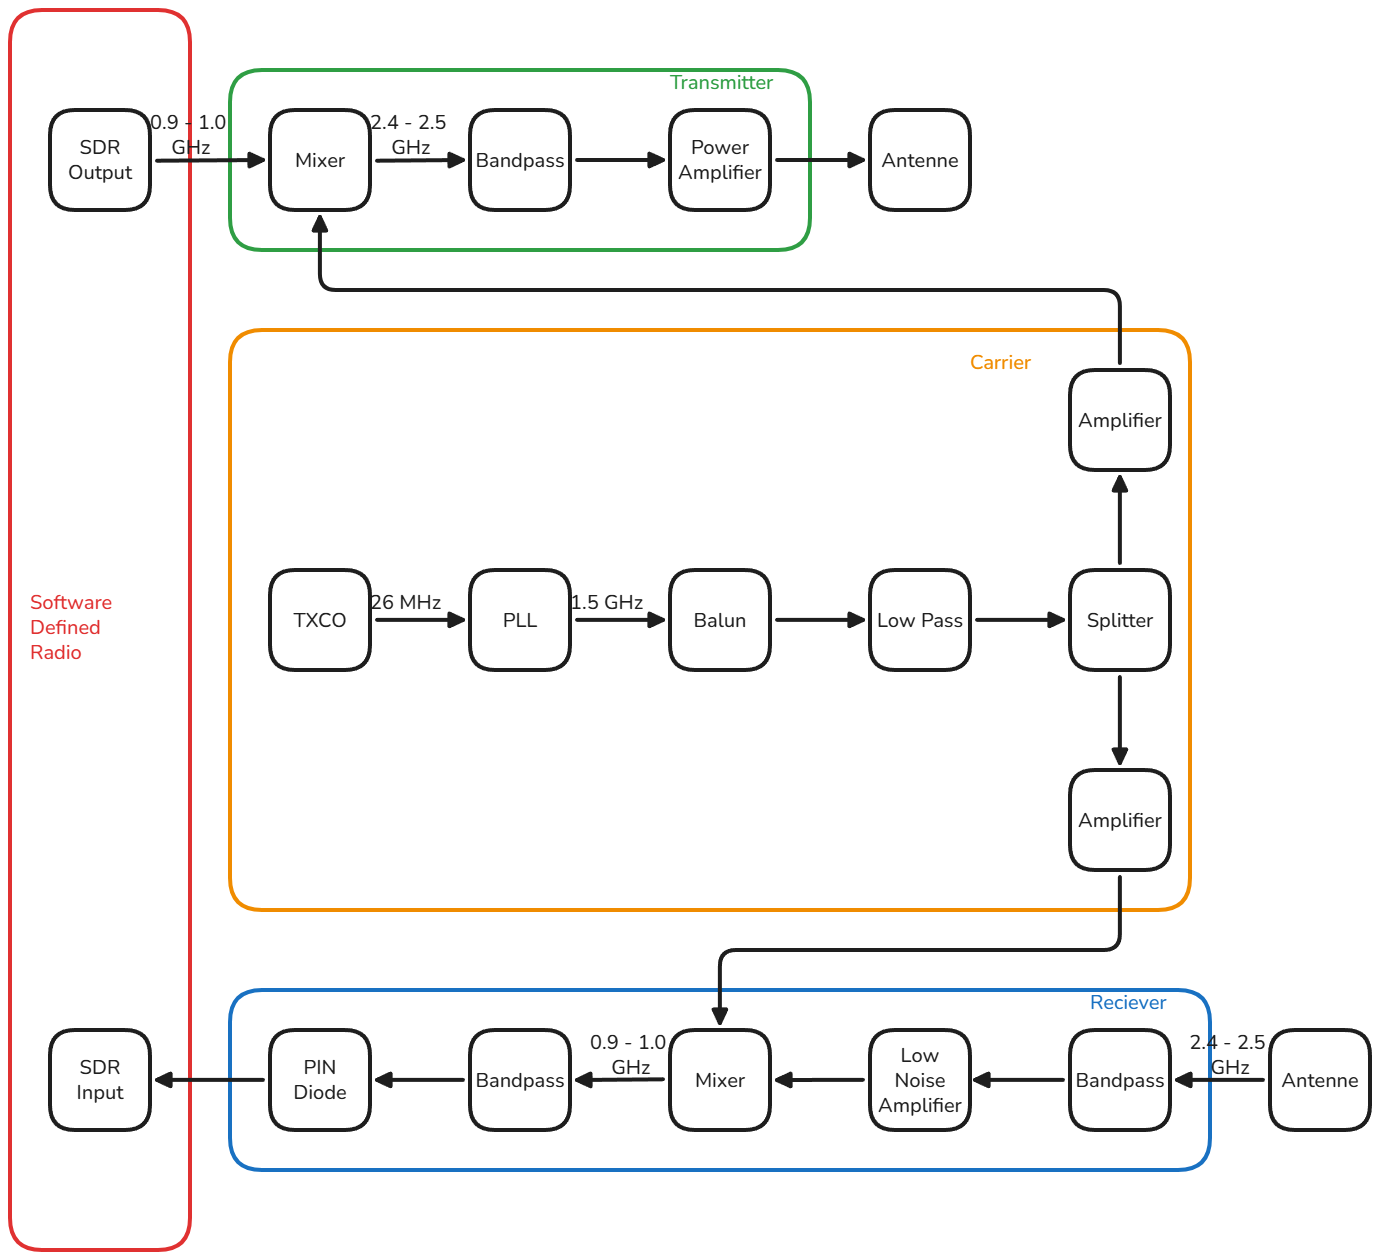
\includegraphics[width=\imagewidthfactor\columnwidth]{media/Blockschaltbild}
    \caption{Blockschaltbild des SDR Frontends.}
    \label{fig:blockschaltbild}
\end{figure}

\section{Oszillator Lösung}

Ein großes Problem war schwer zu lösen und hat daher den Zeitplan gesprengt: für 2.5 GHZ signale mit 900 MHz input ist eine Oszillatorfrequenz von 1.5 GHz notwendig. Kein VCO oder TXO kann diese mit Quatkristallen liefern. 

Mehrer Optionen wurden untersucht:


% TODO: tabelle mit oszillator optionen einfügen

Am ende wurde sich in Absprache mit dem Betreuer auf den PLL geeingigt. Damit stieg die komplexiztät für schematic, layout an. Am meisten wurde damit jedoch die Inbetriebnahme erschwert, da der ADF4351 erst mit einer SPI schnittstelle programmiert werden muss. 